\documentclass[12pt, a4paper]{report}
\usepackage{times}\usepackage{setspace} \doublespacing
% Suport pentru diacritice și alte simboluri
\usepackage{fontspec}

% Suport pentru mai multe limbi
\usepackage{polyglossia}

% Pachet petru afisare pe mai multe coloane
\usepackage{multicol}
% Setează limba textului la română
\setdefaultlanguage{romanian}
% Am nevoie de engleză pentru rezumat
\setotherlanguages{english}

% Indentează și primul paragraf al fiecărei noi secțiuni
\SetLanguageKeys{romanian}{indentfirst=true}

% Suport pentru diferite stiluri de ghilimele
\usepackage{csquotes}

\DeclareQuoteStyle{romanian}
  {\quotedblbase}
  {\textquotedblright}
  {\guillemotleft}
  {\guillemotright}

% Utilizează biblatex pentru referințe bibliografice
\usepackage[
    maxbibnames=50,
    sorting=nty
]{biblatex}

\addbibresource{bibliography.bib}

% Setează spațiere inter-linie la 1.5
\usepackage{setspace}
\onehalfspacing

% Modificarea geometriei paginii
\usepackage{geometry}

% Include funcțiile de grafică
\usepackage{graphicx}
% Încarcă imaginile din directorul `images`
\graphicspath{{./images/}}

% Linkuri interactive în PDF
\usepackage[
    colorlinks,
    linkcolor={blue},
    menucolor={black},
    citecolor={blue},
    urlcolor={blue}
]{hyperref}

% Simboluri matematice codificate Unicode
\usepackage{unicode-math}

% Comenzi matematice
\usepackage{amsmath}
\usepackage{mathtools}

% Formule matematice
\newcommand{\bigO}[1]{\symcal{O}\left(#1\right)}
\DeclarePairedDelimiter\abs{\lvert}{\rvert}

% Suport pentru rezumat în două limbi
% Bazat pe https://tex.stackexchange.com/a/70818
\newenvironment{abstractpage}
  {\cleardoublepage\vspace*{\fill}\thispagestyle{empty}}
  {\vfill\cleardoublepage}
\renewenvironment{abstract}[1]
  {\bigskip\selectlanguage{#1}%
   \begin{center}\bfseries\abstractname\end{center}}
  {\par\bigskip}

% Suport pentru anexe
\usepackage{appendix}

% Pentru descriere
\usepackage{caption}

% Stiluri diferite de headere și footere
\usepackage{fancyhdr}

\fancypagestyle{front}{
  \fancyhf{}
  \renewcommand{\headrulewidth}{0pt}
  \cfoot{}
}
\fancypagestyle{main}{
  \fancyhf{}
  \renewcommand\headrulewidth{0pt}
  \fancyhead[C]{}
  \fancyfoot[C]{\thepage}
}

% Metadate
\title{Detecția de conținut DeepFake cu ajutorul Rețelelor Neuronale Adânci}
\author{Tănase Victor-Flavian}

% Generează variabilele cu @
\makeatletter

\begin{document}

% Front matter
\cleardoublepage
\pagestyle{front}
\let\ps@plain\ps@front

% Pagina de titlu
\begin{titlepage}

% Redu marginile
\newgeometry{left=2cm,right=2cm,bottom=1cm}

\begin{figure}[!htb]
    \centering
    \begin{minipage}{0.2\textwidth}
        
\includegraphics[width=\linewidth]{logo-ub.png}
    \end{minipage}
    \begin{minipage}{0.5\textwidth}
        \large
        \vspace{0.2cm}
        \begin{center}
            \textbf{UNIVERSITATEA DIN BUCUREȘTI}
        \end{center}
        \vspace{0.3cm}
        \begin{center}
            \textbf{
                FACULTATEA DE \\
                MATEMATICĂ ȘI INFORMATICĂ
            }
        \end{center}
    \end{minipage}
    \begin{minipage}{0.2\textwidth}
        
\includegraphics[width=\linewidth]{logo-fmi.png}
    \end{minipage}
\end{figure}

\begin{center}
\end{center}

\vspace{1cm}

\begin{center}
\huge \textbf{\MakeUppercase{Lucrare de licență}}
\end{center}

\vspace{3cm}

\begin{center}
\large \textbf{Absolvent \\ \@author}
\end{center}

\vspace{0.25cm}

\begin{center}
\large \textbf{Coordonator științific \\ Prof. Dr. Radu Ionescu}
\end{center}

\vspace{2cm}

\begin{center}
\Large \textbf{București, iunie 2024}
\end{center}
\end{titlepage}

% Pagina 2 de titlu
\begin{titlepage}

% Redu marginile
\newgeometry{left=2cm,right=2cm,bottom=1cm}

\begin{figure}[!htb]
    \centering
    \begin{minipage}{0.2\textwidth}
        
\includegraphics[width=\linewidth]{logo-ub.png}
    \end{minipage}
    \begin{minipage}{0.5\textwidth}
        \large
        \vspace{0.2cm}
        \begin{center}
            \textbf{UNIVERSITATEA DIN BUCUREȘTI}
        \end{center}
        \vspace{0.3cm}
        \begin{center}
            \textbf{
                FACULTATEA DE \\
                MATEMATICĂ ȘI INFORMATICĂ
            }
        \end{center}
    \end{minipage}
    \begin{minipage}{0.2\textwidth}
        
\includegraphics[width=\linewidth]{logo-fmi.png}
    \end{minipage}
\end{figure}

\begin{center}
\end{center}

\vspace{1cm}

\begin{center}
\huge \textbf{\MakeUppercase{\@title}}
\end{center}

\vspace{3cm}

\begin{center}
\large \textbf{Absolvent \\ \@author}
\end{center}

\vspace{0.25cm}

\begin{center}
\large \textbf{Coordonator științific \\ Prof. Dr. Radu Ionescu}
\end{center}

\vspace{2cm}

\begin{center}
\Large \textbf{București, iunie 2024}
\end{center}
\end{titlepage}

\restoregeometry

\addtocounter{page}{1}

% Rezumatul in limba romana
\begin{abstractpage}

\begin{abstract}{romanian}

Evoluția capabilităților algoritmilor de inteligență artificială din ultimii ani a reinventat crearea de conținut în sfera digitală. În același timp, progresul în câmpul vederii artificiale a fost văzut de către unele entități ca o oportunitate de a răspândi dezinformare sau de a crea conținut malițios greu de detectat cu ochiul liber. 

Ceea ce a început ca cercetare academică realizată de către Justus Thies et al. \cite{thies2016face2face} a dat naștere unui mijloc de fabricare de conținut contrafăcut, capabil să manipuleze imagini și videoclipuri cu un realism nemaivăzut. Acest tip de conținut poate fi folosit in diverse scopuri cu rea-voință precum: șantaj, manipulare politică, înșelătorie, furt de identitate sau creare de conținut neadecvat, de cele mai multe ori aceste atacuri vizând persoane publice. 

În scopul combaterii dezinformării, această lucrare are ca obiectiv punerea la dispoziție către public a unui model de inteligență artificială cu o interfață web, ce poate fi ușor de utilizat pentru detectarea sau cel puțin ridicarea suspiciunii asupra imaginilor sau videoclipurilor posibil fabricate.

\end{abstract}
    
\end{abstractpage}

% Rezumatul in limba engleza
\begin{abstractpage}

\begin{abstract}{english}

The evolution of the artificial intelligence models in recent years has reinvented the creation of content on social media. In the same time, the progress in Computer Vision has been viewed by others as an opportunity to spread misinformation and create malicious content that can be hardly detected by the naked eye.

What has started as academic research by Justus Thies et al. \cite{thies2016face2face} pioneered a new way to fabricate content, capable to manipulate images and videos with unprecedented realism. This type of content can be used in many harmful ways such as blackmailing, political manipulation, fraudulent schemes, identity theft, and the creation of explicit material. Often, public figures are the primary targets of such attacks.

In order to fight disinformation, this work aims to provide the public with an artificial intelligence model with a web interface, that can be easily used to detect or at least raise suspicion over possibly fabricated images or videos. 
\end{abstract}

\end{abstractpage}
\tableofcontents

% Main matter
\cleardoublepage
\pagestyle{main}
\let\ps@plain\ps@main

\chapter{Introducere}

\section{Descrierea problemei}

\section{Motivație}

\section{Contribuție personală}

\section{Privire de ansamblu și organizarea lucrării}

Acest capitol abordeaza conceptele fundamentale care stau la baza înțelegerii rețelelor neuronale. 

\chapter{Concepte Teoretice}

\section{Rețele neuronale}

Rețelele neuronale stau la baza tuturor algoritmilor moderni de inteligență artificială. Acestea au revoluționat industria învățării automate prin puterea lor de a simula funcțiile cognitive ale creierului uman, fiind des folosite in invățarea de tipare(în engleză pattern recognition), diferite sarcini de clasificare si predicție. Ele pot fi văzute ca funcții complicate care primesc date de intrare sub forma unor valori numerice și returnează valori reprezentative pentru acestea. 

\subsection{O scurtă istorie a rețelelor neuronale}

\begin{itemize}
    \item În lucrarea intitulată „A Logical Calculus of the Ideas Immanent in Nervous Activity”(1943) \cite{mcculloch1943logical} Warren McCulloch și Walter Pitts au fost primii care au teoretizat o implementare matematică simplificată a neuronului ca o poartă logică binară. Aceștia au demonstrat teoretic faptul că neuronii au capacitatea de a reprezenta orice funcție matematică.

    \item În 1958, este publicată lucrarea cercetătorului Frank Rosenblatt „The Perceptron: A Probabilistic Model for Information Storage and Organization in the Brain” \cite{rosenblatt1958perceptron}, în care acesta introduce conceptul de Perceptron, cel mai simplu model de rețea neuronală. 

    \newpage
    
    \item Spre finalul anilor 1980, după o lungă perioadă în care studiul rețelelor neuronale a fost neglijat, David E. Rumelhart, Geoffrey Hinton, and Ronald J. Williams (1986) \cite{rumelhart1986learning} prezintă \textbf{backpropagarea}, un algoritm prin care o rețea neuronală putea să învețe eficient, adresând multe dintre problemele ridicate până la acel moment. 

    \item La începutul anilor 2000, tot Geoffrey Hinton, de data aceasta alături de Ruslan Salakhutdinov \cite{hinton2006reducing} aduc o soluție pentru problema gradienților care dispar, prin reducerea dimensionalității datelor.
\end{itemize}

Aceste lucrări din literatură au ajutat la transformarea unor concepte pur teoretice în unelte cu putere de învățare și de decizie care au ajutat la modelarea industriei moderne și au împins progresul tehnologic către noi limite. 

\subsection{De la neuronul biologic la cel artificial}
    La fel ca multe dintre invențiile revoluționare de-alungul istoriei, cercetătorii au avut ca sursă de insipirație viețuitoarele. În cazul inteligenței artificiale, aspirația cercetătorilor a fost să replice neuronul biologic. 
    
    \begin{figure}[h]
         \centering 
         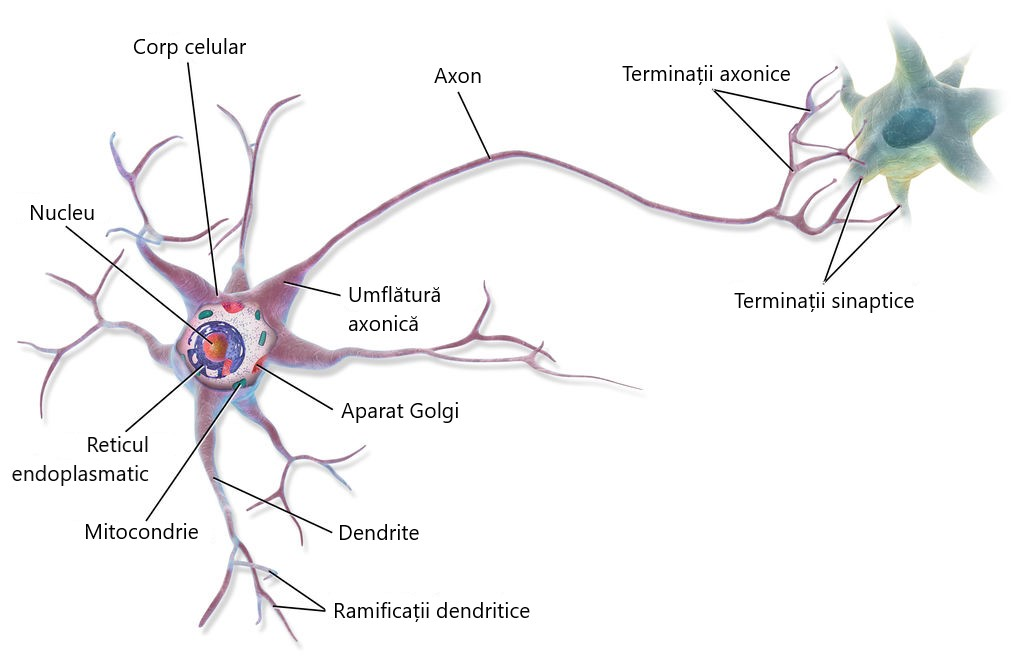
\includegraphics[width=.75\textwidth]{images/structura-unui-neuron.jpg}
         \caption{Anatomia unui neuron \cite{neuron-anatomy}}
    \end{figure}
    
    În zona centrală a neuronului se află corpul celular(soma) care conține nucleul, locul care înmagazineaza tot materialul genetic al celulei. Legate de corpul celular sunt dendritele, care interceptează semnale chimice de la alți neuroni. Atașat de corpul celular, se află o prelungire alungită numită axon, al cărei scop este să transmită semnale electrice către alți neuroni sau către țesuturi. La capătul axonului se găsesc terminațiile acestuia, care sunt legate de dendritele sau de corpul celular ale altui neuron. 

    În creierul biologic, se găsesc miliarde de neuroni, fiecare având mii de legaturi cu alți neuroni aceștia fiind dipusi in straturi pentru a crea țestul nervos. Cu toate că neuronul in sine, nu funcționează intr-un mod complex, ansamblul a miliarde de mecanisme simple într-o rețea imensa are capabilități impresionante. 

    Plecând de la aceste premise Warren McCulloch și Walter Pitts(1943) 
    \cite{mcculloch1943logical} au prezentat în lucrarea lor revoluționară o versiune simplificată a neuronului biologic. Aceștia au văzut neuronul artificial ca o pe poartă logică, cu mai multe intrări și o singură ieșire. Un semnal electric era transmis mai departe doar dacă neuronul avea un număr de intrări care trecea de un anumit prag, bazându-se pe principiul de totul sau nimic al neuronilor biologici.  

     \begin{figure}[h]
         \centering 
         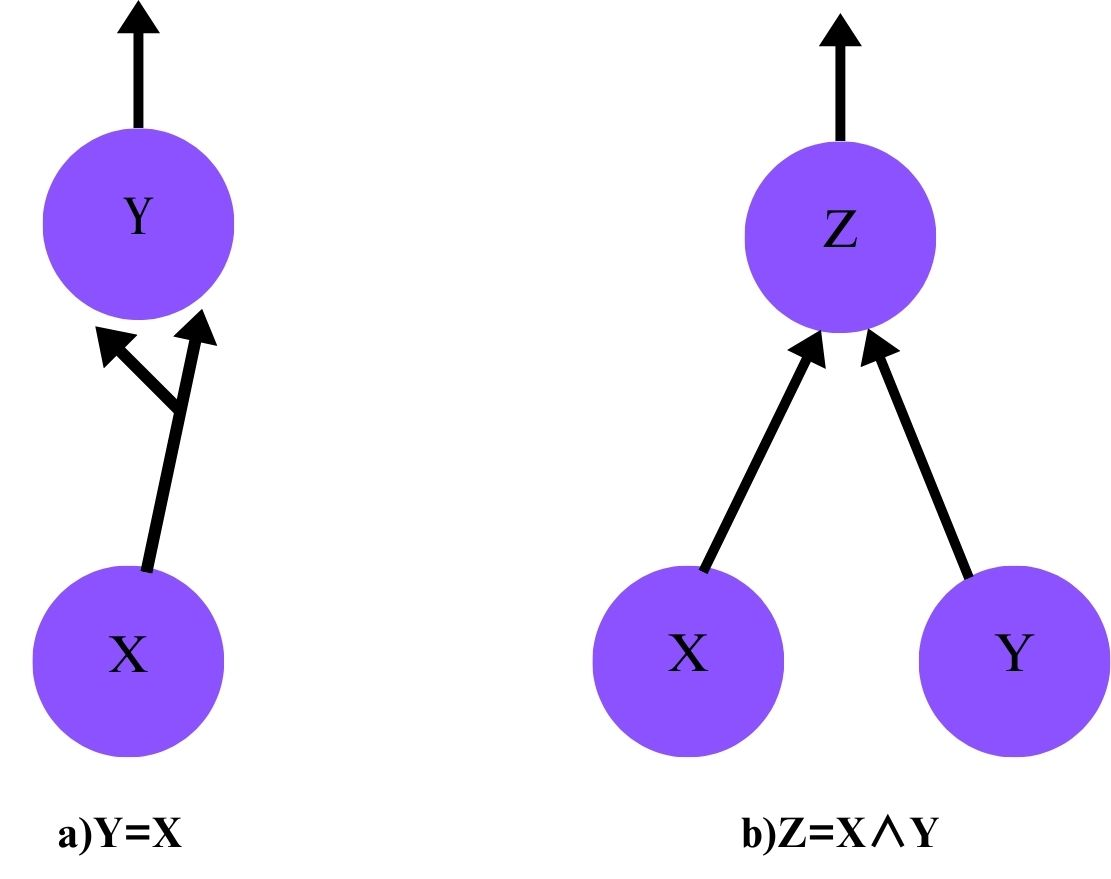
\includegraphics[width=.5\textwidth]{images/artificial-neurons-as-logic-gates.jpg}
         \captionsetup{font=footnotesize}
         \caption{Neuroni artificiali calculând operatii logice}
         \caption*{a) Neuronul Y nu poate transmite semnalul mai departe              doar cu un singur impuls}
         \caption*{b) Neuronul Z are nevoie de ambii neuroni X și Y pentru a trimite un semnal mai departe}
    \end{figure}

    \newpage

\subsection{Perceptronul}

În 1958 Frank Rosenblatt \cite{rosenblatt1958perceptron} introduce in literatură \textbf{perceptronul}, cel mai simplu model de rețea neuronală. Acesta duce neuronul artificial propus de către McCulloch și Pitts \cite{mcculloch1943logical} la un alt nivel. Comparat cu neuronul care transmitea doar semnale binare, cel propus de Rosenblatt este capabil sa proceseze și să transmită mai departe valori numerice. Scopul final este de a organiza aceste unități de calcul într-o „rețea” care primește datele de intrare sub formă numerică și returnează o valoare care le reprezintă. 

Într-o astfel de rețea fiecare neuron se folosește datele de intrare pentru a produce o valoare de ieșire. Fiecărei valori de intrare îi corespunde o pondere(în engleză: weight), un număr real al cărui scop este sa controleze contribuția sa la informația transmisă mai departe de către neuron. Aceste valori sunt însumate ponderat, iar la valoarea obținută se adaugă un neuron special, care la rândul lui are o pondere. Acest neuron se numește \textit{bias}, un număr real, notat cu $b$, care elimină constângerea ca funcția ce reprezintă datele să treacă prin originea planului sau a hiperplanului. Rezultatul reprezintă o funcție care este dată ca parametru unei funcții liniare numită „funcție de pas”(in engleză: step function) pentru a produce valoarea de ieșire a perceptronului. 

\begin{figure}[h]
         \centering 
         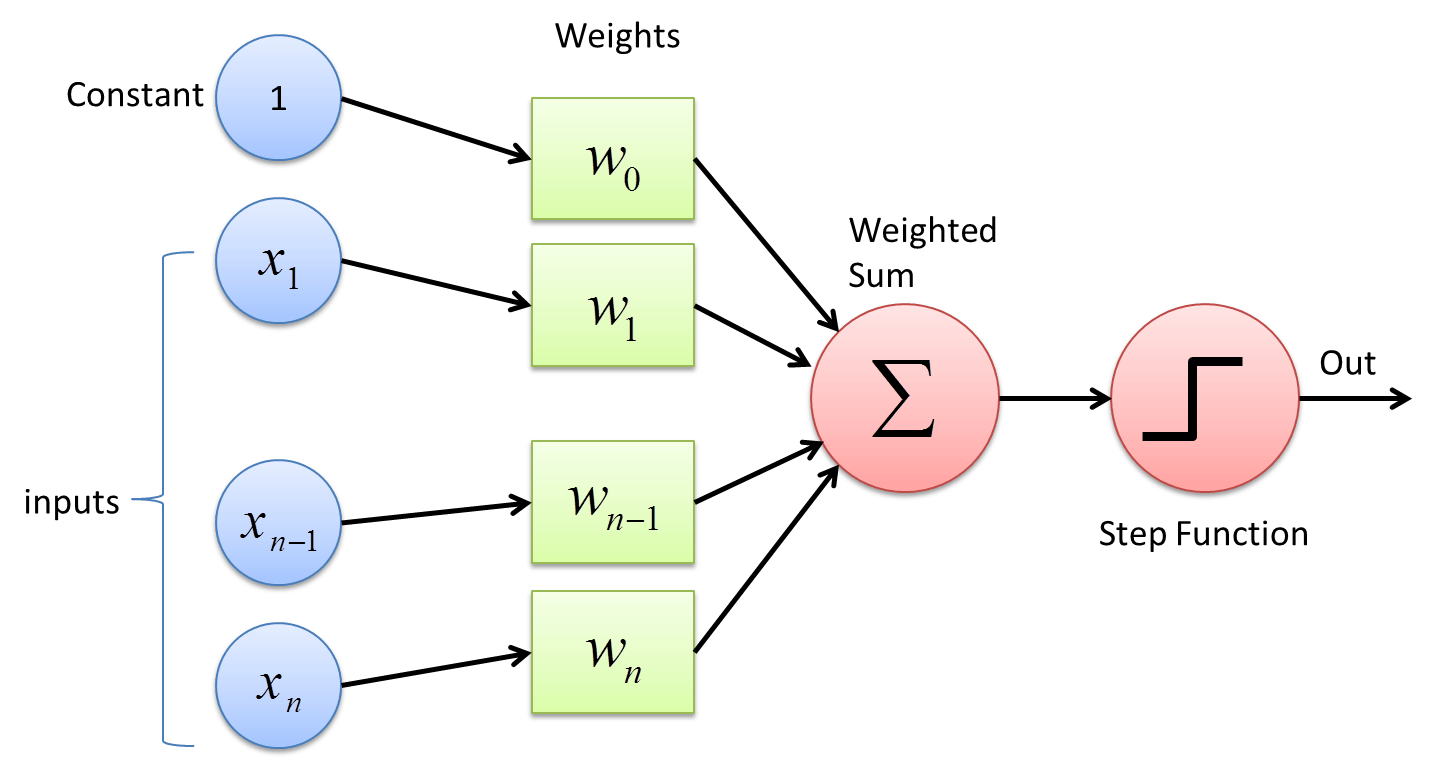
\includegraphics[width=.85\textwidth]{images/the-perceptron.jpg}
         \captionsetup{font=footnotesize}
         \caption{Perceptronul \cite{the-perecptron}}
\end{figure}
\newpage
Notații:

\begin{itemize}
    \item $x = (x_1, x_2, x_3... , x_n)$ datele de intrare
    \item $w = (w_1, w_2, w_3,..., w_n)$ ponderile corespunzătoare 
    \item $b$ = totalitatea neuronilor de \textit{bias} 
    \item $z$ = combinația liniară dintre $x$ si $w$
    \item $z = w_1 x_1 + w_2 x_2 + ... + w_n x_n  = \sum_{i=1}^{n} w_i x_i + b = w^{T}x + b$
    \item $step(z)$ = \textit{output-ul} perceptronului
\end{itemize}
 
O funcție comună folosită drept \textit{step function} este funcția semn definită astfel: 

\[
\text{sgn}(x) = 
\begin{cases} 
    -1 & \text{if } x < 0, \\
    0 & \text{if } x = 0, \\
    1 & \text{if } x > 0.
\end{cases}
\]    

\begin{figure}[h]
         \centering 
         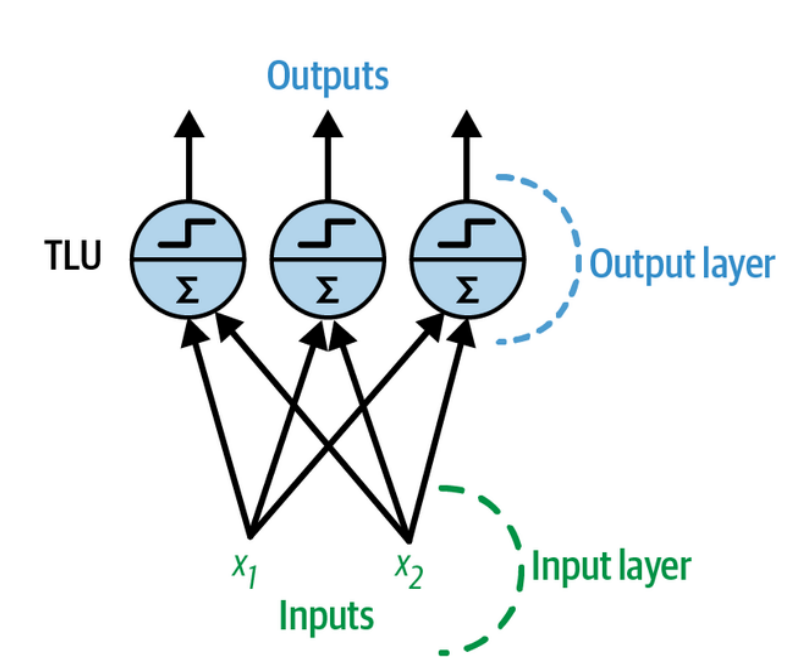
\includegraphics[width=.5\linewidth]{images/multiclass-perceptron.png}
         \captionsetup{font=footnotesize}
         \caption{Un perceptron capabil să separe date în mai multe clase \cite{ageron2019}}
         \label{Figura 2.4}
\end{figure}
\newpage

În Figura~\ref{Figura 2.4} este prezentată o arhitectură de perceptron capabilă sa distingă între 3 clase. Datele de intrare, in cazul nostru $x1$, $x2$ reprezintă \textit{stratul de intrare}. Fiecare valoare din stratul de intrare este legată de toți neuronii din stratul urmator, fiecare legatură având o pondere individuală. Stratul care produce valorile de ieșire se numește \textit{stratul de ieșire} și in exemplul prezentat este format din 3 neuroni, corespunzători fiecărei clasificări posibile. 

În ciuda optimismului declanșat de capabilitățile remarcabile la acea vreme a perceptronului, în 1969 Marvin Minsky și Seymour Papert \cite{minsky1969introduction} au demonstrat limitarea acestui model de a rezolva cateva probleme triviale, precum operația XOR. 

\subsection{Multilayer Perceptron(MLP)}

Soluția pentru limitările perceptronului a fost publicată de David Rumelhart, Geoffrey Hinton și Ronald Williams(1986) \cite{rumelhart1986learning}. Soluția oferita de aceștia a fost unificarea mai multor rețele de tip perceptron intr-o rețea mai mare, numită Multilayer Perceptron(MLP).


\begin{figure}[h]
         \centering 
         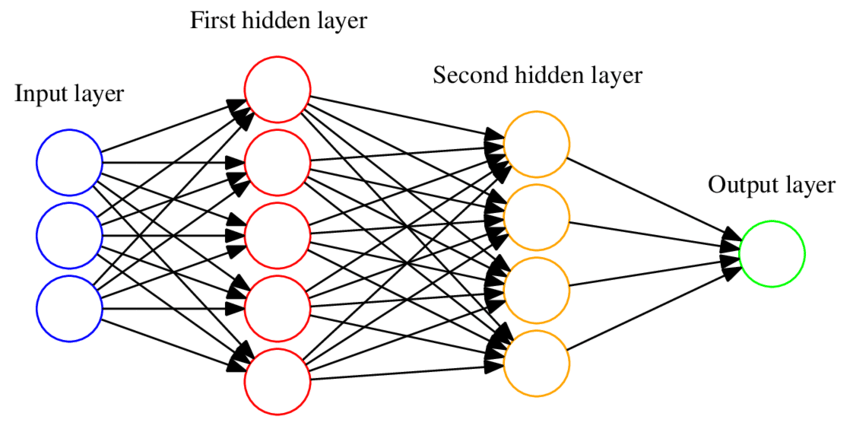
\includegraphics[width=.6\linewidth]{images/MLP.png}
         \captionsetup{font=footnotesize}
         \caption{Arhitectura de tip MLP(Multilayer Perceptron) \cite{phdthesis}}
\end{figure}

\begin{itemize}
    \item Stratul de input = stratul ce conține doar valorile de intrare
    \item Straturile ascunse = straturile prin care se propaga informația. Se sitează între stratul de input și cel de output
    \item Stratul de output = stratul care ne oferă rezultatul trecerii informației prin rețea
\end{itemize}

% \newpage
Arhitectura MLP este una de tip \textbf{feedforward}, cu alte cuvinte, informația se propagă prin rețea intr-o singură direcție, de la stânga la dreapta(dinspre input către output).

În lucrarea lor, cercetătorii au arătat ca rețeaua poate să învețe informații relevante cu ajutorul algoritmului de \textbf{backpropagare}. 
\subsection{Backpropagarea}

Algoritmul prin care o rețea neuronală învață se numește \textbf{backpropagation}. Acesta presupune trecerea prin rețea în repetate rânduri, în doi pași: unul inainte și unul înapoi. Dupa fiecare trecere parametrii(ponderile) sunt actualizați pentru a obține predicții mai bune.
Algoritmul poate fi descris astfel:
\begin{itemize}
    \item Setul de date este spart în blocuri mai mici, cele mai întâlnite dimensiuni fiind de 32, 64 sau 128 de instanțe per bloc
    \item Fiecare bloc este trecut prin rețea: se calculează output-ul primului strat, care este dat ca intrare pentru urmatorul strat, continuând în același fel până se ajunge la stratul de output. Acesta este pasul forward(\textit{forward pass}).
    \item Se evaluează performanța predicțiilor cu ajutorul unei funcții numită \textbf{funcție de pierdere}. Scopul acestei funcții este să furnizeze un scor care să descrie cât de precise au fost predicțiile rețelei față de rezultatul dorit. 
    \item Dupa calculul erorii, algoritmul calculează contribuția fiecărei ponderi din rețea la eroarea totală, cu ajutorul regulii fundamentale din analiza matematică: regula înlănțuirii(în engleză: \textit{chain rule}).
    \item Contribuția la eroarea totală a unui parametru se numește \textbf{gradient}.Valoarea gradientului practic măsoară cât de mult influențează eroarea totală modificarea acelui parmetru.
    \item În cele din urmă, algoritmul folosește gradienții calculați pentru a modifica parametrii cu ajutorul algoritmului coborârii pe gradient.
\end{itemize}
\newpage


\subsection{Algoritmul coborârii pe gradient(\textit{Gradient Descent})}
\label{ch:Gradient Descent}
Coborârea pe gradient este un algoritm iterativ de optimizare, folosit des în literatură, al cărui scop este de găsi minimul global al unei funcții. În cadrul rețelelor neuronale acesta este folosit pentru a optimiza parametrii rețelei astfel încat valoarea erorii totale să se apropie la fiecare iterație de minimul funcției de pierdere. Dupa calcularea gradienților, fiecare pondere se actualizeaza după formula: 
\[
    \scalebox{1.2}{$w_{\text new} = w - \eta \frac{\delta L}{\delta w}$}
\]

Unde: 

\begin{itemize}
    \item $w_{\text new}$ = noua valoare a ponderii
    \item $L$ = valoarea funcției de pierdere
    \item $\frac{\delta L}{\delta w}$ = gradientul 
    \item $\eta$ = rata de învățare(hiperparametru ce controleaza cât de mult se modifică valorile ponderilor)
\end{itemize}

\begin{figure}[h]
         \centering 
         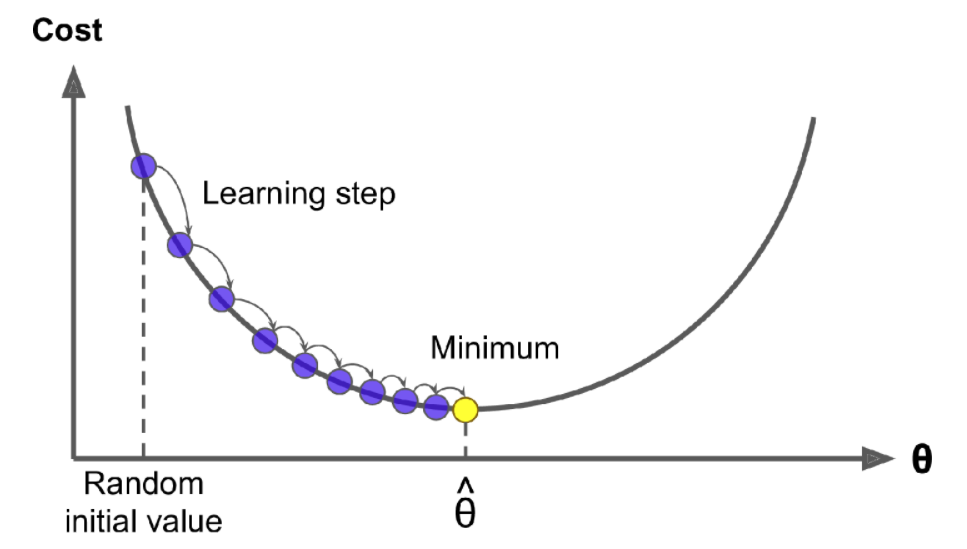
\includegraphics[width=.75\linewidth]{images/gradient-descent.png}
         \captionsetup{font=footnotesize}
         \caption{Vizualizare a algoritmului de coborârii pe gradient \cite{GD}}
\end{figure}
\newpage
Ca backpropagarea să funcționeze Rumelhart et al. au modificat funcția de pas(step function) cu funcția logistică(numită și sigmoidă).
\[
    \scalebox{1.2}{$\sigma(x) = \frac{1}{1 + e^{-x}}$}
\]
Această modificare este esențială deoarece această funcție este diferențiabilă în orice punct, acest lucru ajutând coborârea pe gradient să facă progres la fiecare pas. În urma modificării, denumire de funcție de pas a fost înlocuită de termenul de \textbf{funcție de activare}.

Funcția logistică nu este singura funcție de activare care funcționeaza bine în practică. Alte opțiuni populare în literatură sunt: 
\begin{itemize}
    \item \textbf{tangenta hiperbolică}
    \[
    \scalebox{1.2}{$\tanh(x) = \frac{e^x - e^{-x}}{e^x + e^{-x}}$}
    \]
    \item \textbf{ReLU(Rectified Linear Unit)}
    \[
    \text{ReLU}(x) = 
        \begin{cases} 
        0 & \text{if } x \leq 0 \\
        x & \text{if } x > 0 
        \end{cases}
    \]
    \item \textbf{Leaky ReLU}
    
    \[
    \text{Leaky ReLU}(x) = 
        \begin{cases} 
        \alpha x & \text{if } x < 0 \\
        x & \text{if } x \geq 0 
        \end{cases}
    \]
\end{itemize}

\newpage

\begin{figure}[h]
         \centering 
         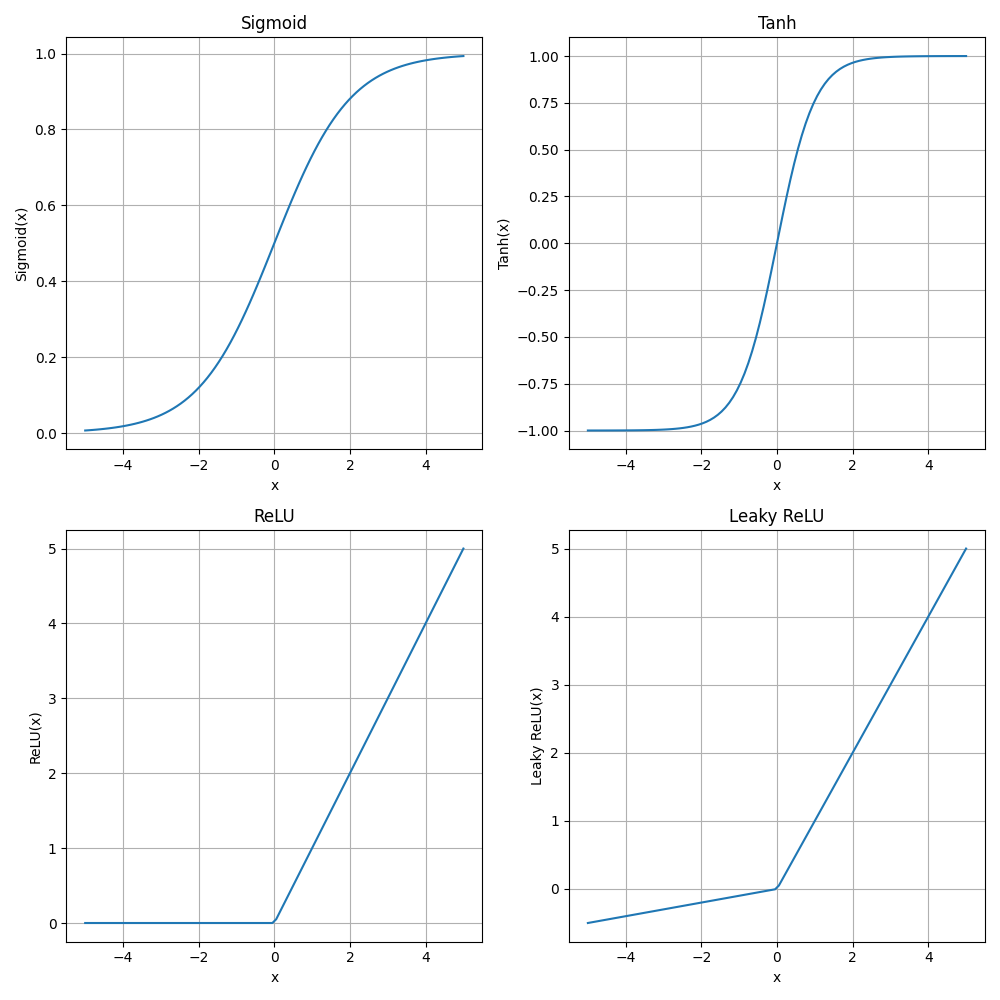
\includegraphics[width=.75\linewidth]{images/activation_functions.png}
         \captionsetup{font=footnotesize}
         \caption{Funcții de activare}
\end{figure}

\subsection{Alți algoritmi de optimizare și optimizarea în practică}

Antrenarea rețelelor neuronale este laborioasă și consumatoare de timp, mai ales pentru seturi voluminoase de date. De aceea, aceasta necesită valori cât mai apropiate de optim pentru hiperparametri, deoarece aceștia controlează antrenarea. 

Un pas important în optimizarea timpului de antrenare este alegerea unei rate de învățare potrivită. O rată de învățare optimă, ajută la reducerea timpului de convergență către optimul global. 

\begin{figure}[h]
         \centering 
         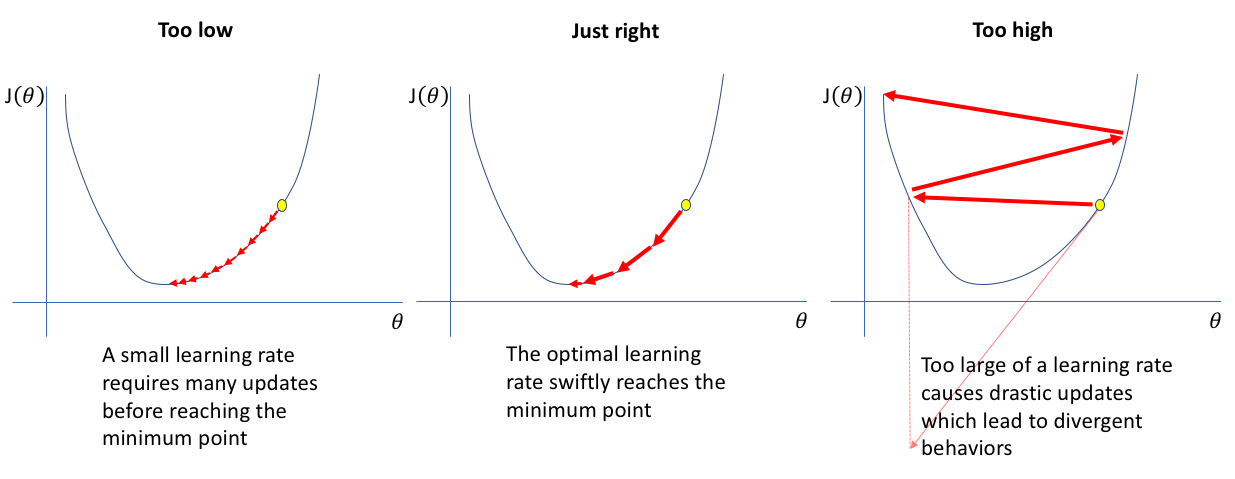
\includegraphics[width=.65\linewidth]{images/learning_rate.png}
         \captionsetup{font=footnotesize}
         \caption{Rata de învățare afectează convergența\cite{learning-rate}}
         \label{Figura 2.7}
\end{figure}
\newpage
În prima imagine din figura \ref{Figura 2.7} se poate observa că o valoare prea mică necesită mai mulți pași pentru a ajunge la convergență. De asemenea, o rată de învățare mică poate determina blocajul într-un minim local. 

În a treia imagine este folosită o rată de invățare prea mare, ceea ce determină divergență(îndepărtarea de minimul global). 

În cea de-a doua imagine pașii sunt mai mari la inceput, iar pe măsură ce pierderea se apropie de minim, pașii devin tot mai mici.

\chapter{Abordări din literatură}
\label{Capitolul 3}
Tehnologia de tip deepfake, ajutată de progresul rapid al modelelor adânci, precum Rețelele Generative Adversariale(GAN), au avut in impact semnificativ în sfera digitală prin crearea de conținut sintetic realistic. Acest avans în tehnologie reprezintă un adevărat pericol pentru confidențialitatea, securitatea și integritatea informației. Din acest motiv, este nevoie de mecanisme robuste pentru detecție a conținutului nelegitim. 

În ultimii ani, diverse lucrări din literatură au abordat această temă folosind inteligență artifcială, dar și tehnici tradiționale bazate pe verificarea inconsistențelor din imagini/videoclipuri. Atenția va fi acordată performanțelor pe bazele de date Celeb-DF \cite{li2020celeb} și FaceForensics++ \cite{rössler2019faceforensics}, întrucât lucrarea prezentată folosește date din aceste două seturi.

\section{Celeb-DF (Celebrities Deepfake)}

Introdusă de Li et al. (2020) \cite{li2020celeb}, Celeb-DF este o bază de date vastă care a devenit un nou etalon pentru detecția de conținut fabricat. A fost proiectată cu scopul de a aduce progres în acest câmp de cercetare, abordând mai multe limitări ale seturilor de date anterioare, precum DeepFakeTIMIT \cite{khan2021adversarially} și FaceForensics++ \cite{rössler2019faceforensics}, oferind videoclipuri deepfake de înaltă calitate și diversitate. Celeb-DF conține 5639 de videoclipuri fabricate de rezoluție înaltă generate folosind o metodă, ce minimizează artefactele de compresie și sporește realismul expressiilor și mișcărilor faciale. 

Un aspect important al acestei baze de date, este faptul că videoclipurile conțin secvențe cu celebrități, un grup de persoane care are șanse mult mai mari să apară în conținut de tip deepfake.

Pe lângă videoclipurile fabricate, setul de date include și un set divers de videoclipuri originale, oferind astfel un mediu de antrenare propice. Intorducerea Celeb-DF a contribuit semnificativ la dezvoltarea tehnicilor de detectare a deepfake-urilor.

\begin{figure}[htbp]
    \centering
    \begin{minipage}[b]{0.45\textwidth}
        \centering
        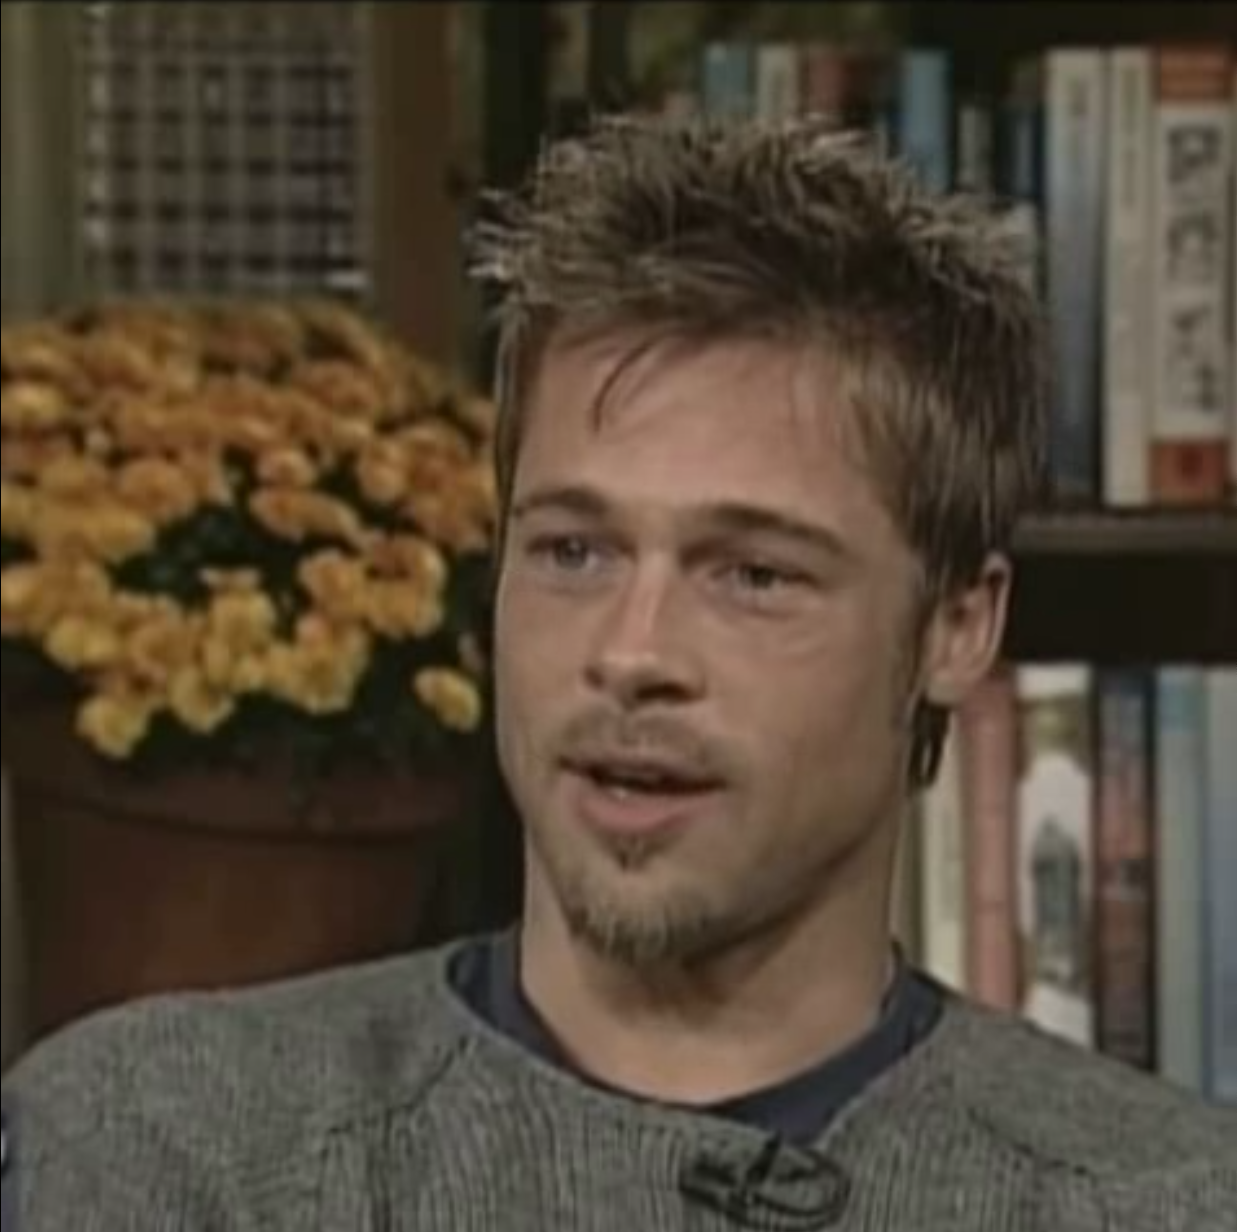
\includegraphics[width=\textwidth]{images/brad-pitt_real.png}
        \caption{Captură dintr-un videoclip original cu actorul Brad Pitt}
    \end{minipage}
    \hfill
    \begin{minipage}[b]{0.45\textwidth}
        \centering
        
\includegraphics[width=\textwidth]{images/brad-pitt_df.png}
        \caption{Captura dintr-un videoclip DeepFake}
    \end{minipage}
\end{figure}

Autorii lucrării au testat riguros pe setul de date diferite modele performante în detecția de deepfake-uri, scoțând în evidență robustețea dar și slăbiciunile lor. Dintre acestea, 2 modele s-au remarcat prin performanța lor.

\begin{itemize}
    \item \textbf{XceptionNet}\cite{rössler2019faceforensics}\cite{Chollet_2017_CVPR}: bazată pe modelul Inception(\cite{szegedy2015going}), această arhitectură s-a dovedit a fi foarte puternică pentru task-uri de clasificare. A fost adaptata pentru detecția de deepfake-uri, datorită capabilităților sale de feature extraction. XceptionNet s-a dovedit a se descurca în particular bine la detecția artefactelor introduse în timpul creării deefake-ului, obținând o acuratețe de 65.5\%.

    \newpage
    \begin{figure}[h]
         \centering 
         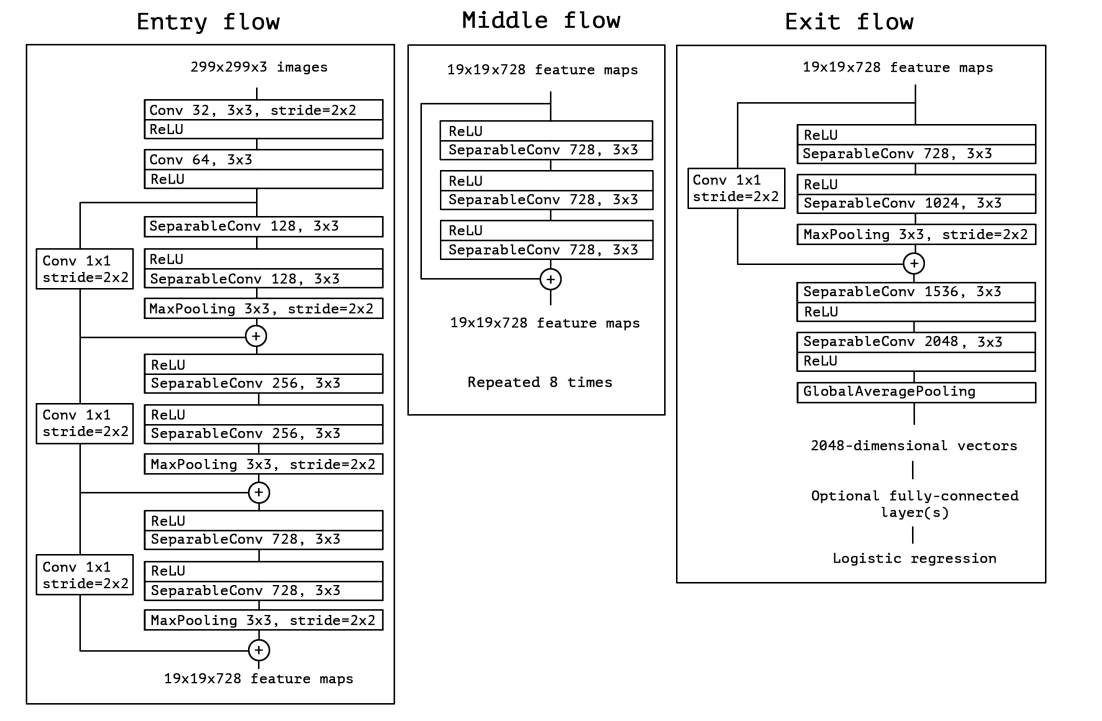
\includegraphics[width=0.85\linewidth]{images/xception-architecture.png}
         \captionsetup{font=footnotesize}
         \caption{Arhitectura Xception \cite{Chollet_2017_CVPR}}
    \end{figure}
    
    \item \textbf{Face Warping Artifacts}\cite{zhou2018twostream}: Modelul Face Warping Artifacts(FWA)este conceput pentru a detecta artefactele de distorsionare a feței, frecvent întâlnite în videoclipurile deepfake. Aceste artefacte sunt distorsiuni subtile introduse în timpul procesului de manipulare a feței, care pot include structura facială nenaturală sau inconsistențe în textură. Combinat cu alte tehnici de detecție a deepfake-urilor, modelul combinat DSP-FWA(DeepFake Stack Pointer Face Warp Artifacts) a obținut o performanță de 64.6\%.
\end{itemize}

\begin{figure}[h]
     \centering 
     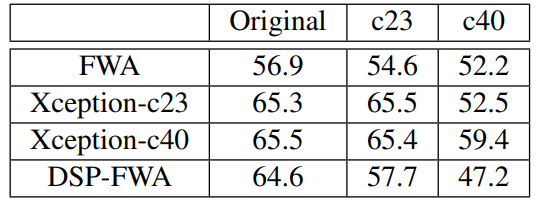
\includegraphics[width=0.5\linewidth]{images/celeb-df_results.png}
     \captionsetup{font=footnotesize}
     \caption{Rezultatele pentru diferite modele \cite{li2020celeb}}
\end{figure}


\section{FaceForensics++}

FaceForensics++ este un set de date și o platformă de benchmark esențială în cercetarea detectării deepfake-urilor și a altor tipuri de conținut deepfake. Dezvoltat de Andreas Rössler și colegii săi, FaceForensics++ a fost conceput pentru a oferi o resursă cuprinzătoare și diversă pentru antrenarea și evaluarea algoritmilor de detectare a conținutului fabricat. 

FaceForensics++ include peste 1,000 de videoclipuri de înaltă calitate, preluate din diferite surse și manipulate folosind mai multe tehnici avansate. Aceste videoclipuri sunt împărțite în patru categorii principale ce reprezintă algoritmii folosiți pentru crearea deepfake-urilor:

\begin{itemize}
    \item \textbf{Deepfakes}: Videoclipuri manipulate folosind tehnici de deepfake, care implică substituirea feței unei persoane cu cea a altei persoane folosind rețele generative adversariale (GANs).
    \item \textbf{Face2Face}\cite{thies2016face2face}:
    \item \textbf{FaceSwap}: Tehnica de schimbare a feței între două persoane în videoclipuri.
    \item \textbf{NeuralTextures}\cite{thies2019deferred}: O metodă care utilizează texturi neurale pentru a asocia expresii faciale sintetice unui model facial.
    
\end{itemize}

\begin{figure}[h]
     \centering 
     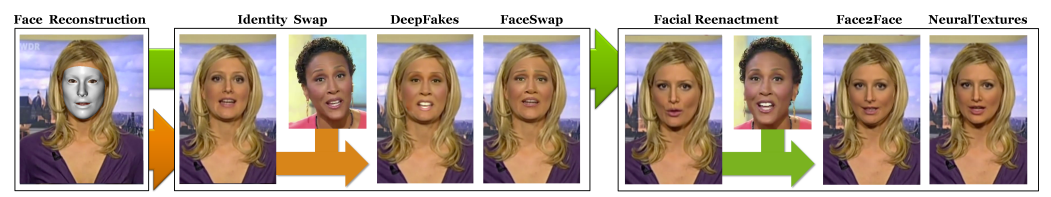
\includegraphics[width=\linewidth]{images/faceforensics.png}
     \captionsetup{font=footnotesize}
     \caption{Procesul de creare a unui DeepFake \cite{rössler2019faceforensics}}
\end{figure}

Setul de date este împărțit în trei subseturi pe baza nivelului de compresie: fără compresie (raw), compresie ușoară (c23) și compresie severă (c40). Acest lucru permite cercetătorilor să testeze robustețea algoritmilor de detecție la diferite niveluri de calitate video.

În lucrarea „Video Face Manipulation Detection Through Ensemble of CNNs”(2020) \cite{bonettini2020video}, autorii abordeaza problema detectării fețelor manipulate în secvențele video, folosind setul FaceForensics++.  Metoda propusă utilizează modelul EfficientNetB4\cite{tan2019efficientnet}, îmbunătățit prin mecanisme de atenție \cite{vaswani2017attention}. Antrenarea modelelor a fost făcută pe seturile de date FaceForensics++ și DeepFake Detection Challenge(o bază de date ce conține peste 119.000 de secvențe din video-uri create pentru o competiție organizată de \href{https://www.kaggle.com/}{Kaggle}. 

\begin{figure}[h]
     \centering 
     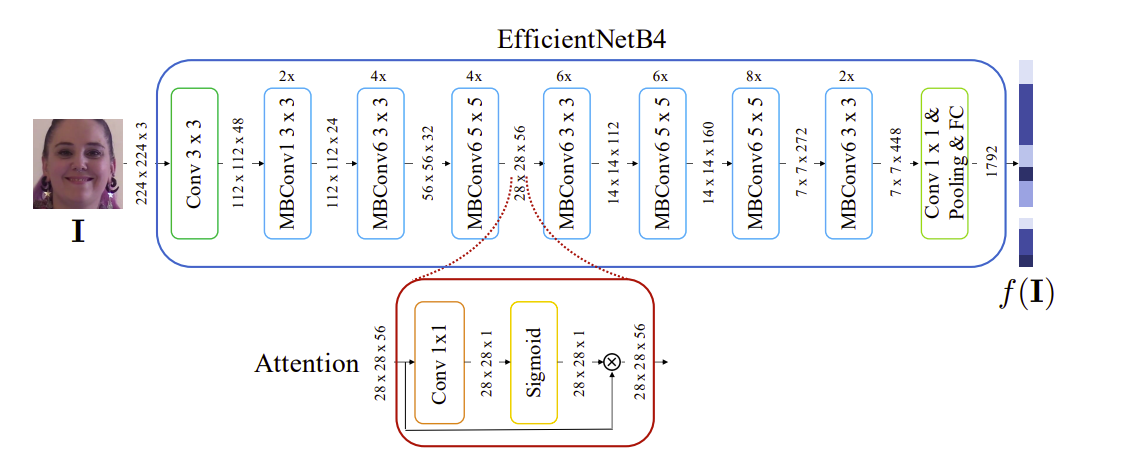
\includegraphics[width=\linewidth]{images/efficientnetb4.png}
     \captionsetup{font=footnotesize}
     \caption{EfficientNetB4 cu atenție \cite{bonettini2020video}}
\end{figure}

Acuratețea modelului a fost evaluată folosind metrica AUC(Area Under Curve), care indică ce capacitate are modelul în a distinge între clasele pozitive și negative.

Autorii au antrenat diverse versiuni ale arhitecturii EfficientNet-B4, pe care în final le-au unit într-un ansamblu de rețele, care a obținut scorul AUC de 0.9444. 


\printbibliography[heading=bibintoc]

\end{document}